\documentclass[10pt,journal]{IEEEtran}
\usepackage[english]{babel}
\usepackage[utf8]{inputenc}
\usepackage[backend=biber]{biblatex}
\usepackage{caption}
\usepackage{graphicx}
\usepackage{float}
\bibliography{referencias}
\begin{document}

\title{Cosmological simulations using a static scalar-tensor theory}

\author{M A Rodríguez-Meza^{1∗}, \ A \ X \ González-Morales^{2}
, \ R \ F \ Gabbasov^{1}
, \ and \ Jorge \ L \ Cervantes-Cota^1 \\
^1Depto. \ de \ Física, \ Instituto \ Nacional \ de \ Investigaciones \ Nucleares, \\
Col. Escandón, Apdo. Postal 18-1027, 11801 México D.F. and \\
^2Departamento \ Ingenierias, \ Universidad \ Iberoamericana, \\
Prol. Paseo de la Reforma 880 Lomas de Santa Fe, Mexico D.F. Mexico \\
^∗mar@nuclear.inin.mx; http://astro.inin.mx/mar \\ (Dated: November 1, 2018)}

\maketitle{}  
%Resumen
\textbf{We present ΛCDM N-body cosmological simulations in the framework of a static general scalartensor theory of gravity. Due to the influence of the non-minimally coupled scalar field, the gravitational potential is modified by a Yukawa type term, yielding a new structure formation dynamics.
We present some preliminary results and, in particular, we compute the density and velocity profiles
of the most massive group.}

\section{INTRODUCTION}
The problem of explaining the structure formation of
the Universe is one of the most fascinating at the beginning of this new millennium. From the recent experimental developments and observations, cosmology has
acquired the status of a high precision area of research
\cite{1}. In fact, recent and independent observational data
measured in the CMBR on various angular scales \cite{2,3}, in
type Ia supernovae \cite{4}, as well as in galaxy surveys \cite{5,6},
suggest that $\Omega=\Omega_\lambda + \omega_m \approx 1$, or that $\Omega_\Lambda \approx 0.73 $ and
$\Omega_m \approx 0.27 $, implying the existence of dark energy and
dark matter, respectively. However, the nature of dark
components is still unknown. These observations favour
the now standard $\Lambda$CDM cosmological model. Despite
some problems on galactic scales revealed by numerical
simulations, which could be explained with some alternative models (e.g. Warm Dark Matter), large scale structure simulations, predicted by the $\lambda$CDM model, agree
well with observations. Naturally, particular inflationary
scenarios motivated by different particle physics theories
have their own dark matter candidates, such as axion,
neutralino, Higgs particle, among others, as well as a
quintessence field \cite{7,8}. In order to include such particles in cosmological models one usually adds a scalar field
(SF) equation to the general relativity field equations.
One possibility is to couple this field non-minimally to
gravity to have a scalar-tensor theory of gravity (STT). \newline
In this work we present some results of the role played
by a massive non-minimally coupled SF on the $\Lambda$CDM
universe structure formation process. Our theoretical
model is built from a general STT static SF which modifies the cosmological dynamics and the Newtonian gravity potential on particles; the dynamical full treatment of
SF perturbations is now under development. We evolve a
cosmological cube using standard $\Lambda$CDM equations with
periodic boundary conditions, where the particles interact through the Newtonian force plus an additional term.
The latter comes from a Yukawa type potential derived
from the Newtonian limit of a STT. It should be noted
that in the present work the SF does not replace the dark
matter or dark energy, but rather coexists with them. To
perform the simulations we have modified a standard serial treecode developed by one of us (MARM) \cite{9} and
Gadget 1 \cite{10} in order to take into account the contribution of the Yukawa potential.

\section{EVOLUTION EQUATIONS USING A STATIC STT}
In a previous paper we found the solutions for the
potential-density pair problem in the Newtonian limit of
a scalar-tensor theory of gravity \cite{11}. Here, we applied
those results and found that the potential of a single particle of mass m is given by \cite{12}
\begin{equation}
    \Phi_N = - \frac{G_N}{1+ \alpha}\frac{m}{r}(1+\alpha e^{-r/\lambda}
\end{equation}

For local scales, $r \ll \lambda$ deviations from the Newtonian
theory are exponentially suppressed, and for $r \gg \lambda$the
Newtonian constant diminishes (augments) to $G_n/(1+\alpha)$ for positive (negative) $\alpha$. This means that equation
(1) fulfills all local tests of the Newtonian dynamics, and
it is only constrained by experiments or tests on scales
larger than –or of the order of –$\lambda$, which in our case is of
the order of galactic scales.
To simulate cosmological systems, the expansion of the
Universe has to be taken into account. Here, we employ a
cosmological model with a static scalar field which is consistent with the Newtonian limit given by Eq. (1). Thus,
the scale factor, $a(t)$, is given by the following Friedman
model,

\begin{equation}
    a^3H^2=H_{0}^{2} \left[\frac{\Omega_{m0}+\Omega_{\Lambda 0}a^3}{1+\alpha}+\left(1-\frac{\Omega_{m0}+\Omega_{\Lambda 0}}{1+\alpha}\right)\alpha \right]
\end{equation}

where $H=\Dot{a}/a$, $\Omega_{m0}$ and $\Omega_{\Lambda 0}$ are the matter and energy
density evaluated at present, respectively. We notice that
the source of the cosmic evolution is deviated by the term
1+$\alpha$ when compared to the standard Friedman-Lemaitre
model. Therefore, it is convenient to define a new density parameter by $\Omega_{i}^{\alpha}\equiv \Omega_i / (1+\alpha)$. This new density parameter is such that $\Omega_{m}^{\alpha}+\Omega_{\Lambda}^{\alpha}=1$, which implies a
flat Universe, and this shall be assumed in our following
computations, where we consider $(\Omega_{m}^{\alpha},\Omega_{\Lambda}^{\alpha})=(0.3,0.7)$.
For positive values of $\alpha$, a flat cosmological model demands to have a factor (1 + $\alpha$) more energetic content
($\Omega_m$ and $\Omega_\Lambda$) than in standard cosmology. On the other
hand, for negative values of $\alpha$ one needs a factor (1 + $\alpha$)
less $\Omega_m$ and $\Omega_\Lambda$ to have a flat Universe. To be consistent with the CMB spectrum and structure formation
numerical experiments, cosmological constraints must be
applied on $\alpha$ in order for it to be within the range (−1, 1)
\cite{13,14,15,16}.
In the Newtonian limit of STT of gravity, the Newtonian motion equation for a particle $i$ is written as

\begin{equation}
    \Ddot{x_i}+2Hx_i=-\frac{1}{a^3}\frac{G_N}{1+\alpha}\sum_{j\neq i}\frac{m_j(x_i-x_j)}{|x_i-x_j|^3}F_{SF}(|x_i-x_j|,\alpha,\lambda)
\end{equation}
where x is the comovil coordinate, and the sum includes
all periodic images of particle j, and $F_{SF}(r,\alpha,\lambda)$ is

\begin{equation}
    F_{SF}(r,\alpha,\lambda)=1+\alpha \left(1+\frac{r}{\lambda} \right) e^{-r/\lambda} 
\end{equation}

which, for small distances compared to $\lambda$, is $F_{SF} (r <
\lambda, \alpha, \lambda) \approx 1 + \alpha (1+\frac{r}{\lambda})$
and, for long distances, is
$F_{SF} (r > \lambda, \alpha, \lambda) \approx 1$, as in Newtonian physics. \newline
We now analyze the general effect that the constant
$\alpha$ has on the dynamics. The role of α in our approach
is as follows. On one hand, to construct a flat model
we have set the condition $\Omega_{m}^{\alpha}+\Omega_{\Lambda}^{\alpha}=1 $, which implies
having (1 + $\alpha$) times the energetic content of the standard $\Lambda$CDM model. This essentially means that we have
an increment by a factor of (1 + $\alpha$) times the amount
of matter, for positive values of $\alpha$, or a reduction of the
same factor for negative values of $\alpha$. Increasing or reducing this amount of matter affects the matter term on
the r.h.s. of the equation of motion (3), but the amount
affected cancels out with the term (1 +$\alpha$) in the denominator of (3) stemming from the new Newtonian potential
(1). On the other hand, the factor FSF augments (diminishes) for positive (negative) values of $\lambda$ for small distances compared to $\lambda$, resulting in more (less) structure
formation for positive (negative) values of α compared to
the $\Lambda$CDM model. For $r\gg \lambda$ the dynamics is essentially
Newtonian.
\section{RESULTS}

We now present results for the ΛCDM model of the
Universe model previously described. Because the visible component is the smaller one and given our interest
to test the consequences of including a SF contribution
to the evolution equations, our model excludes gas particles, but all its mass has been added to the dark matter. Therefore, our model is as follows. We start our
simulation with an initial distribution of $N = 2 × 32^3$
particles in a box with sides of $50h^{−1}$ Mpc at z = 10. \newline
This case is similar to the one that comes with Gadget 1
[10]. At present epoch,$\Omega_{b0}^{\alpha}=0$, $\Omega_{m0}^{\alpha}=0.3$, $\Omega_{\Lambda 0}^{\alpha}=0.7$, $H_0=100h \ km/s/Mpc$, $h=0.7$. We restrict the values of $\alpha$ to the interval (−1, 1) [13, 14, 15, 16] and use $\lambda$ = 5
Mpc, since this scale turns out to be an intermediate scale
between the size of the clump groups and the separation
of the formed groups. \newline
In Fig. \ref{f:1} we show $y–z$ snapshots at redshift $z$ = 0 of
our $\Lambda$CDM model. Fig. \ref{f:1} (a) presents the standard case
without SF, i.e., the interaction between bodies through
the standard Newtonian potential. In (b) we show the
case with $\alpha$ = 1, $\lambda$ = 5 Mpc. In (c) $\alpha$ = −1/2, $\lambda$ = 5
Mpc. In (d) $\alpha$ = −1/4, $\lambda$ = 5 Mpc. One notes clearly
how the SF modifies the matter structure of the system.
The most dramatic cases are (b) and (c) where we have
used $\alpha$ = 1 and $\alpha$ = −1/2, respectively. Given the argument at the end of last section, in the case of (b),
for $r \ll \lambda$ the effective gravitational pull has been augmented by a factor of 2, in contrast to case (c) where
it has diminished by a factor of 1/2; in model (d) the
pull diminishes only by a factor of 3/4. That is why one
observes for $r$ < $\lambda$ more structure formation in (b), less
in (d), and lesser in model (c). The effect is then, for a
growing positive $\alpha$, to speed up the growth of perturbations, then of halos and then of clusters, whereas negative
$\alpha$ values ($\alpha \rightarrow$ -1) tend to slow down the growth. \newline
Next, we found the groups in the system using a friendof-friend algorithm and select one of the most massive
ones. The chosen group is located approximately at y =
19 Mpc, $z$ = 12 Mpc, and it is labeled with the letter “G”
in Fig. 1(a). The group was analyzed by obtaining their
density profiles and circular velocities. In Fig. 2(a) we
show the density profiles for this group. The more cuspy
case is for $\alpha$ = 1 and the less cuspy is for $\alpha$ = -1/2.\newline
In Fig. 2(b) we show, for the same group, circular
velocity curves, computed using $v_{c}^{2}=G_NM(r)/r$. The
case with $\alpha$ = 1 corresponds to higher values of vc, since
this depends on how much accumulated mass there is at
a distance r and this is enhanced by the factor FSF for
positive values of $\alpha$. \newline
The groups are at most 2 Mpc in size at z = 0, which
means that the inner structure is such that r < $\lambda$, being
affected by the factor FSF as explained at the end of
section 2. While for r > $\lambda$ the overall structure formation
process is governed by Newtonian physics, which is the
reason why the overall structure of the models in Fig. \ref{f:1}
is similar.

\section{CONCLUSIONS}

We have used a general, static STT that is compatible
with local observations by the appropriate definition of
the background field constant, i.e. $<\phi>=G_N^{-1}(1+\alpha)$.
A direct consequence of our approach is that the amount
of matter (energy) has to be increased for positive values
of $\alpha$ and diminished for negative values of $\alpha$ with respect
to the standard $\Lambda$CDM model in order to have a flat cosmological model. Quantitatively, our model demands to
have $\Omega/(1+\alpha)=1$ and this changes the amount of dark
matter and energy of the model for a flat cosmological
model, as assumed. \newline

\begin{figure}[H]
    \centering
    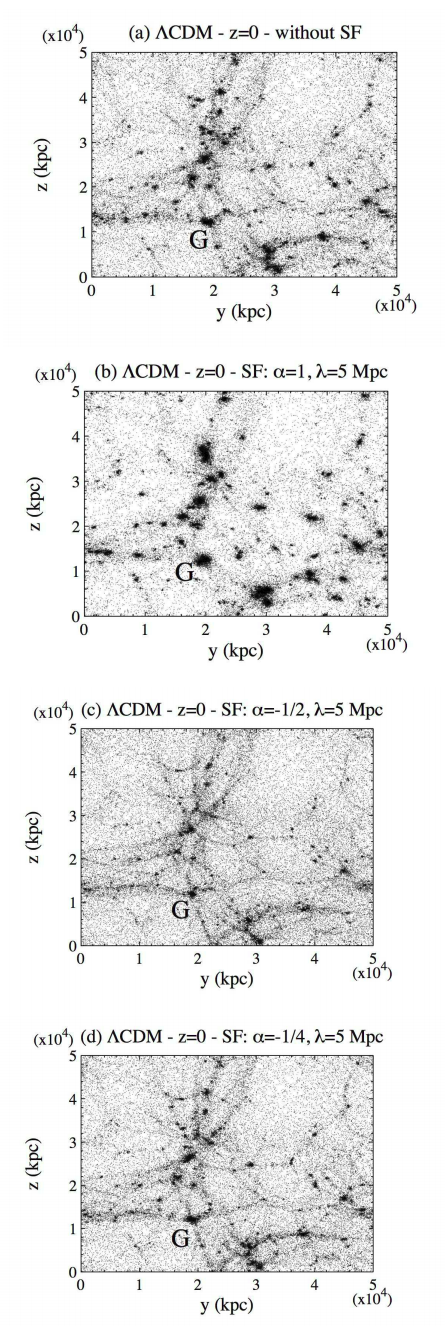
\includegraphics[scale=0.5]{img/alma 1.png}
    \caption{ y–z snapshots at $z$ = 0 of a $\Lambda$CDM universe. See text
for details.}
    \label{f:1}
\end{figure}

\begin{figure}[H]
    \centering
    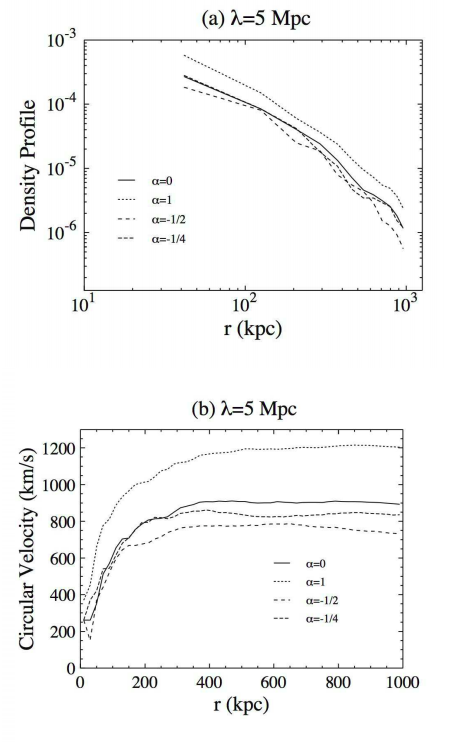
\includegraphics[scale=0.55]{img/alma 2.png}
    \caption{ (a) Density profiles for one of the most massive groups
at $z$ = 0 of a $\Lambda$CDM universe. The group is located approximately at $y$ = 19 Mpc, $z$ = 12 Mpc, labeled with “G” in Fig
1(a). Vertical scale is in units of $\rho_0=10^{10}M_{\bigodot}h^{-1}/(h^{-1}kpc)^3$.
(b) The corresponding circular velocity.}
    \label{f:2}
\end{figure}

The general gravitational effect is that the interaction
including the SF changes by a factor $F_{SF}(r,\alpha,\lambda) \approx1+\alpha(1+\frac{r}{\lambda})$ for $r$ < $\lambda$ in comparison with the Newtonian case. Thus, for $\alpha$ > 0 the growth of structures speeds up
in comparison with the Newtonian case. For the $\alpha$ < 0
case the effect is to diminish the formation of structures.
For r > $\lambda$ the dynamics is essentially Newtonian. \newline
Using the resulting modified dynamical equations, we
have studied the structure formation process of a $\Lambda$CDM
universe. We varied the amplitude and sign of the
strength of the SF ($\alpha$) in the interval (-1,1) and performed several 3D-simulations with the same initial conditions. From our simulations with different values of $\alpha$,
we have found that the inclusion of SF changes local dynamical properties of the most massive group considered,
and accordingly the density profile and circular velocity,
however, the overall structure is somewhat similar. Here,
we notice that we have also studied other massive groups,
in particular one smaller group located approximately at
$y$ = 16.5 Mpc, $z$ = 22 Mpc in Fig. 1(a). The trends
are quite similar to the most massive group, so that our
conclusions prevail.
In this work we only varied the amplitude of the SF
($\alpha$) leaving the scale length ($\lambda$) of the SF unchanged.
After some preliminary runs, the increase of $\lambda$ enhances
the structure formation process for $\alpha$ positive, and the decrease of $\lambda$ makes the structure grow at a slower rate. \newline
In a future work we will study an ampler space parameter
and with a much better resolution. Also, the cosmological initial conditions will be constructed using the matter
density field corresponding to the modified gravity. \newline
\newline\newline\newline\newline\newline\newline
Acknowledgements: This work was supported by
CONACYT, grant number I0101/131/07 C-234/07, IAC
collaboration. The simulations were performed in the
UNAM HP cluster Kan-Balam.

\printbibliography[title={BIBLIOGRAPHY}]

\end{document}
